\documentclass[linenumbers]{aastex631}

\newcommand{\vdag}{(v)^\dagger}
\usepackage{multirow}
\usepackage{booktabs}
\usepackage{graphicx}
\graphicspath{ {./Figures/} }
\usepackage{subfigure}
\usepackage{float}
\usepackage{microtype}
\usepackage{natbib}
\usepackage{url}
\usepackage{makecell}
\usepackage{array}
\usepackage{tabularx}
\usepackage[english]{babel}

\makeatletter
\let\frontmatter@title@above=\relax
\makeatother

\begin{document}

\title{V765 Cas: A Fortuitous Eclipsing Binary in the Owl Cluster}

\newcommand\SOHS{Stanford Online High School \\ Redwood City, CA, USA}
\author{Jacob Bryant}
\affiliation{\SOHS}

\author{Sabine Mazzeo}
\affiliation{\SOHS}

\author{Thomas Morford}
\affiliation{\SOHS}

\author{Elle Moscinski}
\affiliation{\SOHS}

\author{Kalée Tock}
\affiliation{\SOHS}

\begin{abstract}
This is the abstract
\end{abstract}
\keywords{TODO}

\section{Introduction}
\label{sec:intro}

abcd

\begin{figure}[H]
\centering
\plotone{Final-Image-Calibrated-for-Reddening.jpg}
\caption{Composite color image of NGC 457 (Shown and discussed later, included here for visual).} 
\label{fig:calimg}
\end{figure}

abcd


\begin{table}[H]
\centering
\caption{Information about the system from VSP and GDR3. \label{tabgeninfo}}
\begin{tabular}{ | c | c | c | c | c | c | }
    \hline
    Name & Coordinates & PM (Ra, Dec) (mas/y) & \makecell{Magnitude \\ Range (V)} & Distance (pc) \\
    \hline
    \hline
    V765 Cas & \makecell{01 19 09.05 \\ +58 17 26.0} & \makecell{-1.726 ± 0.140, \\ -0.686 ± 0.130} & 10.60 - 11.23 & 2948 \\
    \hline
    \makecell{HD 236689 \\ (Comp 95)}  & \makecell{01 18 33.08 \\ +58 22 30.5} & \makecell{-1.762 ±0.010, \\ -0.779 ±0.012} & 9.386 & 2856 \\
    \hline
    \makecell{NGC 457 100 \\ (Comp 106)} & \makecell{01 19 46.44 \\ +58 12 26.0} & \makecell{-1.510 ±0.011, \\ -0.702 ±0.014} & 10.601 & 2680 \\
    \hline
\end{tabular}
\end{table}

Next is the table about something

\begin{table}[H] 
\caption{V765 Cas and Comp Star Magnitudes in Filters Used. \label{tabmagsinfo}}
\centering
\begin{tabular}{ | c | c | c | c | }
    \hline
    Name &
        Source &
        Filter &
        Magnitude \\
    \hline
    \hline
    %\multirow{3}{*}{V765Cas} & 
    %    \multirow{3}{*}{GDR3} &
    %    \\
    V765Cas  &
        GDR3 & G & 10.620233\\ \cline{3-4}
        { }  & { } & B\_BP & 10.771473 \\ \cline{3-4}
        { }  & { } & G\_RP & 10.324134 \\
    \hline
    Comp95  &
        APASS &
        V & 9.386 \\ \cline{3-4}
        { }  & { } & B & 9.731 \\ \cline{3-4}
        { }  & { } & SG & 9.507 \\ \cline{3-4}
        { }  & { } & SR & 9.365 \\ \cline{3-4}
        { }  & { } & SI & 9.356 \\
    \hline
    Comp 106 &
        APASS &
        V & 10.601 \\ \cline{3-4}
        { }  & { } & B & 10.906 \\ \cline{3-4}
        { }  & { } & SG & 10.744 \\ \cline{3-4}
        { }  & { } & SR & 10.553 \\ \cline{3-4}
        { }  & { } & SI & 10.547 \\
    \hline
\end{tabular}
\end{table}


\section{Instruments Used}
\label{sec:instr}

\section{Plots}
\label{sec:plots}

\begin{figure}[H]
\centering
%\plotone{Figures/Ratio-of-Comps-106-v.-95-SI.png}
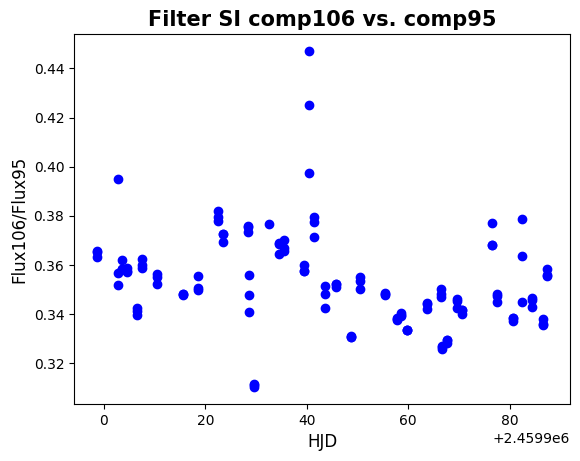
\includegraphics[width=10cm]{Ratio-of-Comps-106-v.-95-SI.png}
\caption{Flux ratio of comp stars 106 and 95 in SI filter.} 
\label{fig:ratiocompssi}
\end{figure}

\begin{figure}[H]
\centering
%\plotone{Figures/Comp-106-Calibrated-Mag-SI.png}[width=6cm]
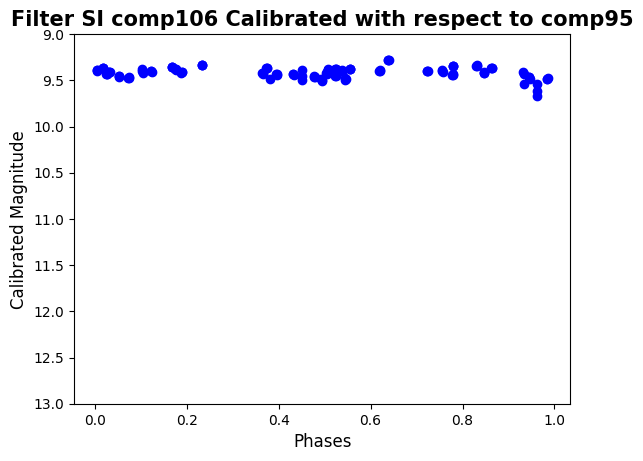
\includegraphics[width=10cm]{Figures/Comp-106-Calibrated-Mag-SI.png}
\caption{Calibrated magnitude of Comp 106 with respect to Comp 95 in the SI filter versus phase.} 
\label{fig:comp106sicalmag}
\end{figure}

\begin{equation} \label{eqcalmag}
\text {mag} _ {\text {calibrated}} = \text {mag} _ {\text {comp117}} - 2.5 \times \log \left( \frac {\text {flux} _ {\text {target}}} {\text {flux} _ {\text {comp117}}} \right)
\end{equation}

\begin{figure}
\plotone{Figures/V765Cas-Lightcurve-All-Filters-Stacked.png}
\caption{Combined light curve of V765 Cas in B, V, SG, SI, and SR filters.} 
\label{fig:allfilterlightcurve}
\end{figure}

\begin{figure}[H]
\centering
%\plotone{Figures/V765Cas-ASAS-SN-Lightcurve.png}
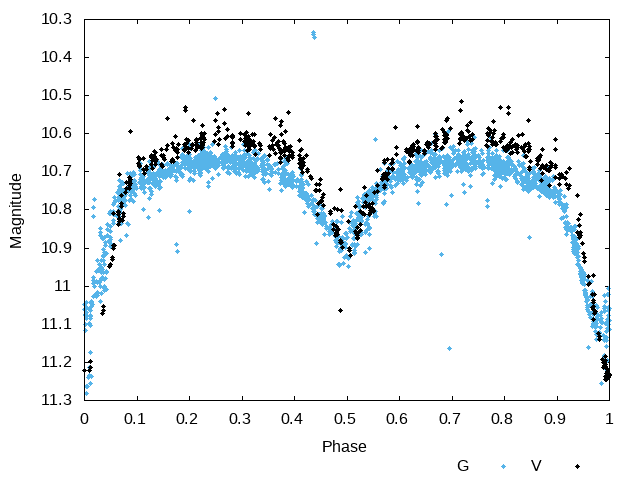
\includegraphics[width=10cm]{Figures/V765Cas-ASAS-SN-Lightcurve.png}
\caption{ASAS-SN light curve of V765 Cas.} 
\label{fig:asassnlightcurve}
\end{figure}

\begin{figure}[htb!]
  \centering
  \begin{subfigure}{}
    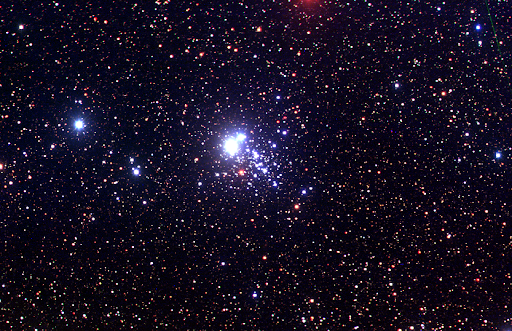
\includegraphics[width=2.5in]{Figures/NGC457-Composite-Image-withSU.png}
  \end{subfigure} 
  \begin{subfigure}{}
    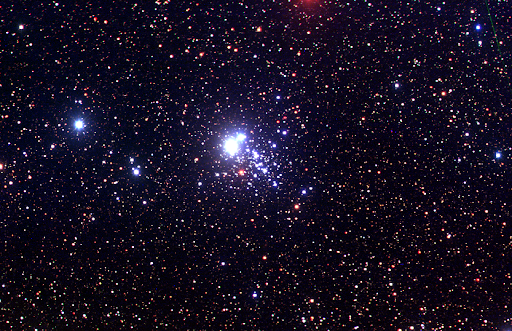
\includegraphics[width=2.5in]{Figures/NGC457-Composite-Image-withoutSU-withRcorrec.png}
  \end{subfigure}
  \label{colorcomposites}
  \caption{Composite color images of NGC 457 with the SU filter (left) and without the SU filter and with reddening correction (right)}
\end{figure}

\begin{figure}[htb!]
\centering
%\plotone{Figures/V765Cas-ASAS-SN-Periodogram.png}
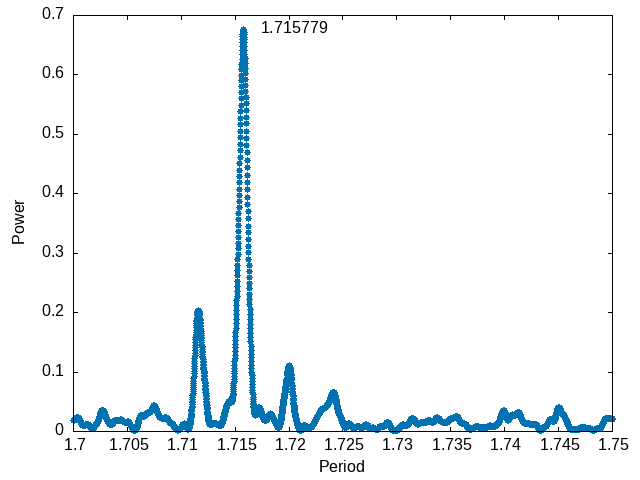
\includegraphics[width=10cm]{Figures/V765Cas-ASAS-SN-Periodogram.png}
\caption{Periodogram of ASAS-SN Photometry of V765 Cas.} 
\label{fig:asassnperiodogram}
\end{figure}

\begin{figure}[htb!]
  \centering
  \begin{subfigure}{}
    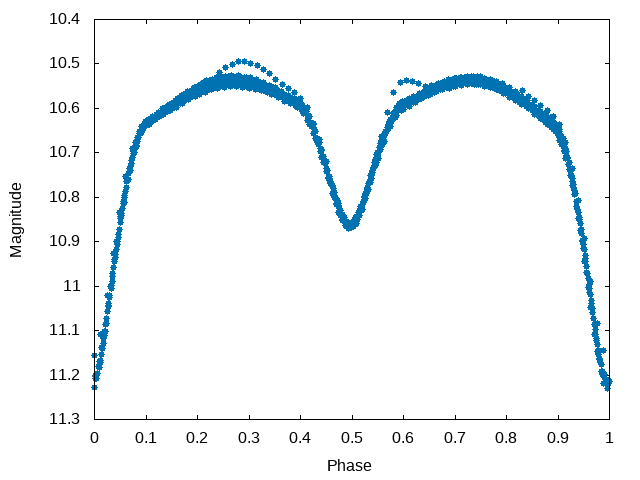
\includegraphics[width=2.5in]{Figures/V765Cas-TESS-CDIPS-Lightcurve.png}
  \end{subfigure} \\
  \begin{subfigure}{}
    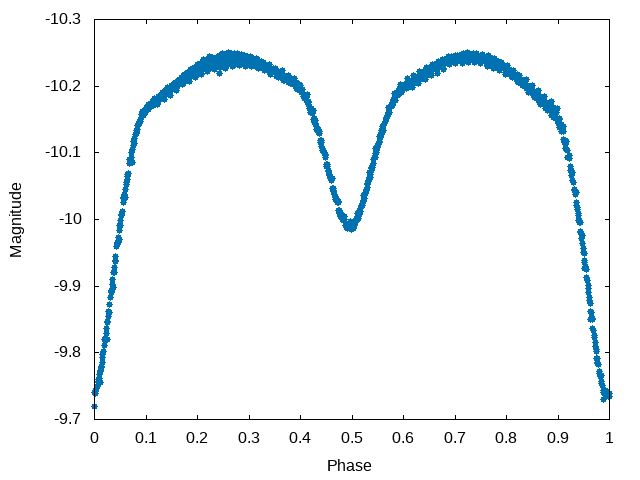
\includegraphics[width=2.5in]{Figures/V765Cas-TESS-PATHOS-Lightcurve.png}
  \end{subfigure}
  \begin{subfigure}{}
    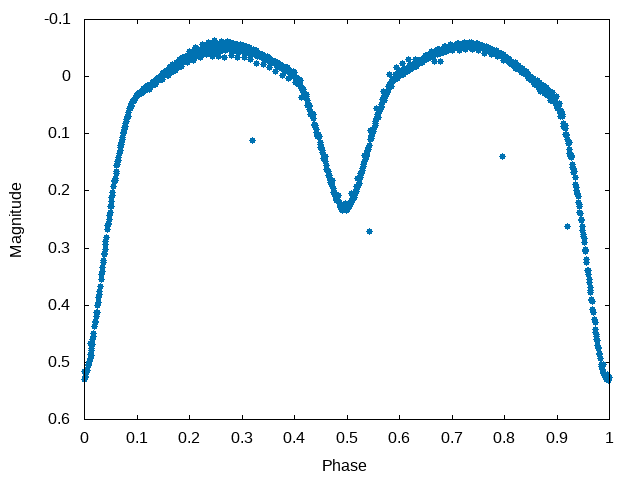
\includegraphics[width=2.5in]{Figures/V765Cas-TESS-QLP-Lightcurve.png}
  \end{subfigure}
  \caption{Light curves from the TESS CDIPS (top), PATHOS (left), and QLP (right) pipelines.}
  \label{fig:tesslightcurves}
\end{figure}

\begin{figure}[H]
\plotone{Figures/Isochrone-Final-Cropped.png}
\caption{Isochrone of NGC 457.} 
\label{fig:isochrone}
\end{figure}

\begin{table}[H]
\caption{Information from the Isochrone. \label{tabisoinfo}}
\begin{tabular}{ | c | c | c | c | c | }
    \hline
     Source & Distance (kpc) & Reddening (mag) & Metallicity ($M_{\bigodot}$) & Log Age (log year) \\
    \hline
    \hline
    Isochrone &  3.65 ± 1.24 & 0.4 & -0.4 & 7.324 \\
    \hline
    WEBDA & 2.429 & 0.472 & --- & 7.324 \\
    \hline
\end{tabular}
\end{table}

\section{Conclusion}
\label{sec:concl}
This study demonstrates that a set of images can have many uses and data extracted from them—aside from being images of a beautiful cluster. From the images of the NGC 457 cluster, we were able to photometrically study V765 Cas, an EA-type binary with a period of 1.715779 days (which although is approximately 7 seconds greater than the previous measurement, is within the realm of uncertainty, thus still reinforcing the known period).

After calibrating the magnitudes from different instruments’ images using non-variable comp stars, we produced light curves from the 5 filters—SG, SI, SR, V, and B—of AAVSOnet images of the NGC 457 cluster. Light curves were also made from TESS and ASAS-SN data to support the validity of the light curves. Additionally, we made a composite color image of the cluster, and an isochrone.

The light curve in Fig. \ref{fig:allfilterlightcurve} (Section \ref{sec:plots}) shows two distinguishable eclipses in all 5 filters, the primary eclipse in which there is approximately a 0.8 drop in magnitude, and the secondary, in which the magnitude drops by a little under 0.4 (though the exact magnitude drop depends on the filter). It can thus be inferred that, since the primary and secondary eclipses are clear and distinct, and cause different amplitude dips, the system V765 Cas is in fact an EA-type eclipsing binary. 

\section{Future Work}
\label{sec:fut}
Continuing to work with V765 Cas, more information can be extracted from the images. In particular, one could do a color analysis of the photometry as each eclipse is happening. Since we have the images in several filters, it is possible to check if the light dips in a unique way in one filter during an eclipse in a way that it does not in another filter. This could allow one to learn more about the two individual stars and their composition.

The process we used to study V765 Cas can then be applied to other fortuitous variable stars. Even in the field of the NGC 457 cluster, there are at least 31 confirmed variable stars \citep{MACIEJEWSKI}—this is a rich starfield, and there are countless more studies to be done.


\begin{acknowledgments}
\section{Acknowledgments}
We acknowledge with thanks the variable star observations from the AAVSO International Database contributed by observers worldwide and used in this research.
\newline \newline
Special thanks goes to the volunteer site managers at the AAVSOnet observatories: Walt Cooney at the Madrona Peak Observatory and Arne Henden at the BSM New Hampshire II Observatory.
\newline \newline
This publication makes use of data products from APASS, funded by the Robert Martin Ayers Sciences Fund and the National Science Foundation.
\newline \newline
This research has made use of the International VSX database, operated at AAVSO, Cambridge, Massachusetts, USA.
\newline \newline
Astropy (Price-Whelan et al, 2022), SciPy (Virtanen and Gommers, 2020), NumPy (Harris, 2020), Pandas (McKinney, 2010) and IPython (Pérez and Granger, 2007) were used in the creation of the plots.
\newline \newline
Dr. Bob Buchheim at AAVSO graciously helped in the process of accessing TESS light curves.
\newline \newline
The cfitsio program (W. Pence 1999) was used to manipulate FITS files.
\newline \newline
This work has made use of data from the European Space Agency (ESA) mission Gaia (http://www.cosmos.esa.int/gaia), processed by the Gaia Data Processing and Analysis Consortium (DPAC, http://www.cosmos.esa.int/web/gaia/dpac/consortium). Funding for the DPAC has been provided by national institutions, in particular the institutions participating in the Gaia Multilateral Agreement.
\newline \newline
This research has made use of PYTHON code written by Daryl Janzen at the University of Saskatchewan for plotting a light curve using ASAS-SN data.
\newline \newline
This research has made use of the SIMBAD database, operated at CDS, Strasbourg, France, and the “Aladin Sky Atlas” developed at CDS, Strasbourg Observatory, France.
\newline \newline
This research has made use of Dan Reichart's Skynet Plotting tool (https://skynet.unc.edu/ASTR101L/graph/).
\newline \newline
This paper includes data collected with the TESS mission, obtained from the Mikulski Archive for Space Telescopes (MAST) data archive at the Space Telescope Science Institute (STScI). The TESS mission is an MIT-led NASA mission, funded by the NASA Explorer Program. STScI is operated by the Association of Universities for Research in Astronomy, Inc., under NASA contract NAS 5–26555.
\newline \newline
This research has made use of the VizieR catalog access tool, CDS, Strasbourg, France (DOI: 10.26093/cds/vizier). The original description of the VizieR service was published in 2000, A\&AS 143, 23.
\newline \newline
This research has made use of the WEBDA database, operated at the Department of Theoretical Physics and Astrophysics of the Masaryk University. 

Funding for the Sloan Digital Sky Survey V has been provided by the Alfred P. Sloan Foundation, the Heising-Simons Foundation, the National Science Foundation, and the Participating Institutions. SDSS acknowledges support and resources from the Center for High-Performance Computing at the University of Utah. The SDSS web site is \url{www.sdss.org}.

SDSS is managed by the Astrophysical Research Consortium for the Participating Institutions of the SDSS Collaboration, including the Carnegie Institution for Science, Chilean National Time Allocation Committee (CNTAC) ratified researchers, the Gotham Participation Group, Harvard University, Heidelberg University, The Johns Hopkins University, L’Ecole polytechnique fédérale de Lausanne (EPFL), Leibniz-Institut für Astrophysik Potsdam (AIP), Max-Planck-Institut für Astronomie (MPIA Heidelberg), Max-Planck-Institut für Extraterrestrische Physik (MPE), Nanjing University, National Astronomical Observatories of China (NAOC), New Mexico State University, The Ohio State University, Pennsylvania State University, Smithsonian Astrophysical Observatory, Space Telescope Science Institute (STScI), the Stellar Astrophysics Participation Group, Universidad Nacional Autónoma de México, University of Arizona, University of Colorado Boulder, University of Illinois at Urbana-Champaign, University of Toronto, University of Utah, University of Virginia, Yale University, and Yunnan University.

\citep{vsp} exists.
\citep{SDSS} exists.

\end{acknowledgments}
\facilities{TODO}
\software{list any}

%\begin{thebibliography}{2}
%\bibliographystyle{aasjournal.bst}

%\end{thebibliography}

%\bibliography{refs}

\appendix

\section{Appendix A} \label{appa}
Although each filter started with a slightly different number of images per filter, this was especially true after we sorted every image to discard compromised ones, as described in Section \ref{sec:plots}. The final values of the number of images used in our analysis is in Table \ref{tab:numimg}

\begin{table}[H]
    \centering
    \begin{tabular}{ | c | c | c | }
    \hline
        Filter & Comp106 & Comp95 \\ \hline \hline
        SU & 81 & 81 \\ \hline
        SG & 81 & 81 \\ \hline
        SI & 121 & 124 \\ \hline
        SR & 80 & 81 \\ \hline
        ZS & 51 & 78 \\ \hline
        B & 44 & 44 \\ \hline
        V & 42 & 42 \\ \hline
        R & 45 & 45 \\ \hline
    \end{tabular}
    \caption{Number of images in which comp stars are found per filter.}
    \label{tab:numimg}
\end{table}

\section{Appendix B} \label{appb}

\noindent
Historically stars were cataloged into six magnitude categories, with category 1 being the brightest and category 6 being the dimmest, a convention created by Hipparchus (Hughes 2006). Later, in 1856, Norman R. Pogson introduced a logarithmic scale for magnitudes (Hughes 2006). He decided that a star of magnitude m is exactly $10^{\frac 2 5}$ brighter than one of magnitude $m+1$. In other words, this means that a star of magnitude 1 is 100 times brighter than a star of magnitude 6 (as $(10^{\frac 2 5})^5 = 100$, the 5 being because there are 5 ‘steps’ between a magnitude 1 and 6 star)
\newline \newline
In astronomy, flux is defined as the amount of energy/light received from the star divided by area of the receiver. When using the same images (or more specifically, the same telescope that thus has the same receiving area), a ratio of fluxes is essentially just brightness as the areas cancel. 
\newline \newline
Due to Pogson’s definition that became convention, a star of magnitude $m=6$ has flux $f_m$ that is 100 times smaller than the flux $f_n$ of a star of magnitude $n=1$. This can be written as: 

\begin{equation}
    \frac{f_n}{f_m} = 100 ^ {(\frac{m-n}{5}} = (10^2 )^ {(\frac{m-n}{5})}
\end{equation}
Then one can take the log of both sides and simplify using the exponent rule: 

\begin{equation}
    \log(\frac {f_n} {f_m}) = \log(10^2) ^ {((m-n)/5)} = (\frac{2*(m-n)}5)*\log(10) = (\frac{2*(m-n)}5)*1= \frac 2 5 (m-n)
\end{equation}
Or in shorter form: 

\begin{equation} \label{eqd3}
    \log(\frac {f_n} {f_m}) = \frac 2 5 (m-n)
\end{equation}
Then dividing the left side by $\frac 2 5$ gives

\begin{equation}
    \log (\frac {f_n} {f_m}) / (\frac 2 5) = \frac 5 2 \log (\frac {f_n} {f_m})
\end{equation}
And therefore \ref{eqd3} can be rewritten as this:

\begin{equation}
    2.5 \log (\frac {f_n} {f_m}) = m-n
\end{equation}
The negative is just due to the fact that we tend to write it as the star that is in the numerator of flux ratio is the first one in the difference (so $n-m$ instead of $m-n$ like we have here), so just simple rearranging.

\begin{equation}
    n-m = -2.5 \log (\frac {f_n} {f_m})
\end{equation}
Thus we obtain our final calibrated magnitude equation (\ref{eqcalmag}) by assigning $n$ to the target and $m$ to the comp: 

\begin{equation}
    \text {mag} _ {\text {calibrated}} = \text {mag} _ {\text {comp117}} - 2.5 \times \log \left( \frac {\text {flux} _ {\text {target}}} {\text {flux} _ {\text {comp117}}} \right) 
\end{equation}


\section{Appendix C} \label{appc}
Figure \ref{fig:compratio} below shows the graphs of the ratio of flux of the chosen comp star combination, 106 and 95, in all the filters we have. Figure \ref{fig:calcomp106} below shows the graphs of the calibrated magnitude of comp 106 with respect to comp 95 in all the available filters (SG, SR, SI, B, and V) versus the phase of the images of the comp stars used. Table [TODO STDEV] shows the standard deviation that ratio for all comp star combinations and in all filters and the mean standard deviation across all filters used for each pair of comp stars used.

\begin{figure}[H]
\centering
%\plotone{Figures/Ratio-of-Comps-106-v.-95-Mag-All-Filters.png}
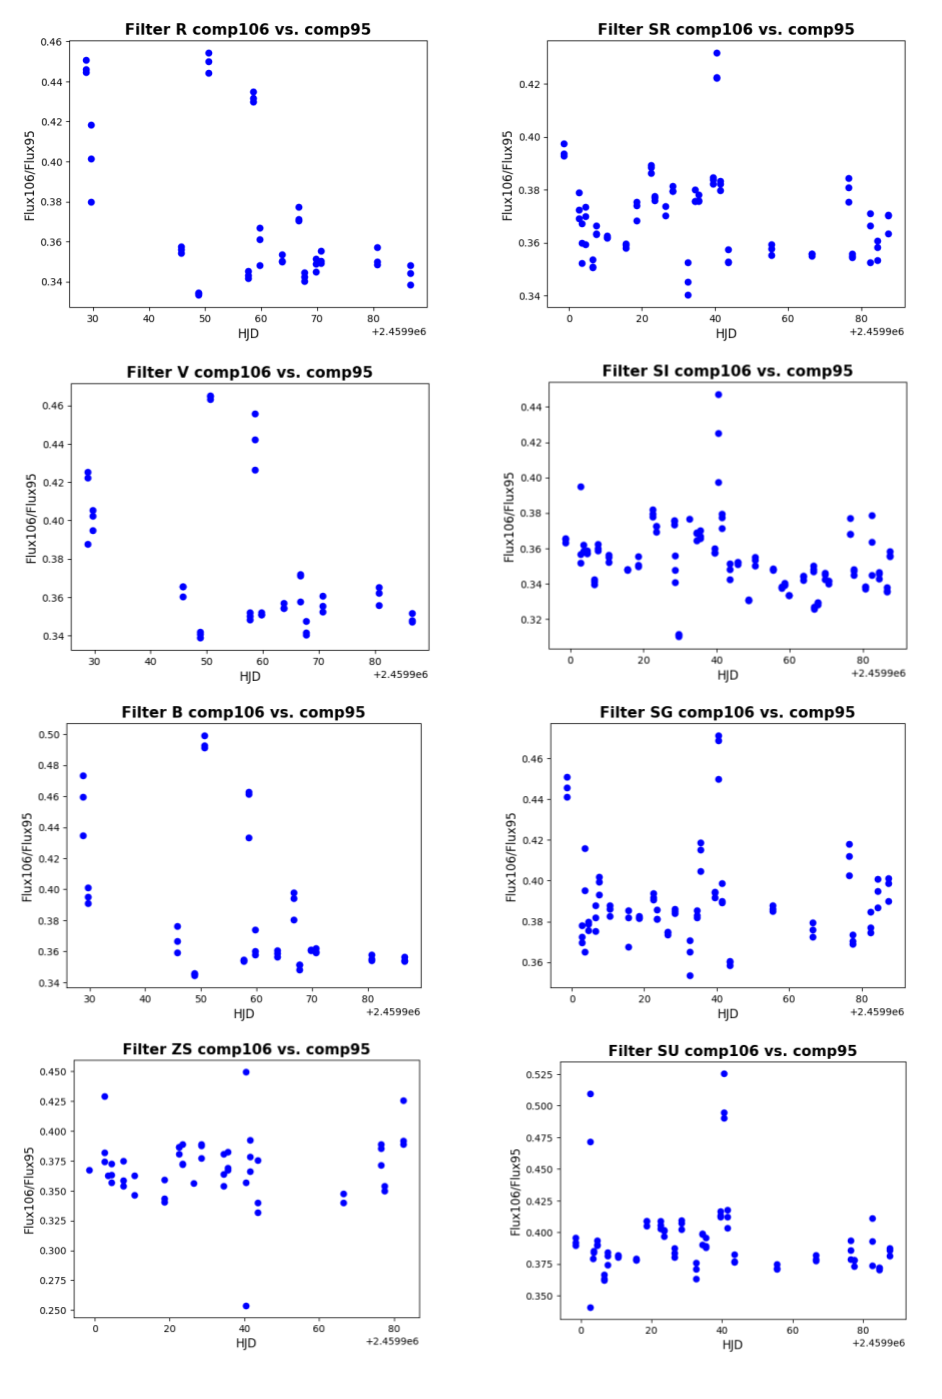
\includegraphics[width=15cm]{Figures/Ratio-of-Comps-106-v.-95-Mag-All-Filters.png}
\caption{Ratio of comp star 106 v. 95 magnitude in all filters used.} 
\label{fig:compratio}
\end{figure}

\begin{figure}[H]
\plotone{Figures/Calibrated-Magnitude-of-Comp-106.png}
\caption{Calibrated magnitude of comp106 with respect to comp95 v. phase in SG, SR, SI, B, and V filters.} 
\label{fig:calcomp106}
\end{figure}

\begin{table}[H]
    \centering
    \begin{tabular}{ | c || c | c | c | c | c | c | }
    \hline
        {} & 117 v. 111 & 117 v. 106 & 116 v. 95 & 111 v. 106 & 111 v. 95 & 106 v. 95 \\ \hline \hline
        SG & 0.026985 & 0.018726 & 0.006507 & 0.020309 & 0.008858 & 0.022691 \\ \hline
        SI & 0.022976 & 0.024631 & 0.005640 & 0.033490 & 0.009864 & 0.019401 \\ \hline
        SR & 0.020690 & 0.017600 & 0.004328 & 0.024164 & 0.008940 & 0.016487 \\ \hline
        SU & 0.065299 & 0.013345 & 0.003179 & 0.012269 & 0.003170 & 0.030756 \\ \hline
        V & 0.017183 & 0.006467 & 0.015508 & 0.024172 & 0.030863 & 0.037934 \\ \hline
        B & 0.020583 & 0.010090 & 0.020473 & 0.014698 & 0.018673 & 0.045446 \\ \hline
        R & 0.013270 & 0.008960 & 0.017229 & 0.033169 & 0.042396 & 0.038874 \\ \hline
        ZS & 0.070951 & 0.054620 & 0.019086 & 0.079086 & 0.018591 & 0.027586 \\ \hline \hline 
        Mean value & 0.032242 & 0.019305 & 0.01149375 & 0.030170 & 0.017669 & 0.029897 \\ \hline
    \end{tabular}
    \caption{Flux ratio standard deviation of comp star combination vs. filter.}
    \label{tab:stdevfluxcomps}
\end{table}

\section{Appendix D} \label{appd}
Figure \ref{fig:indivlightcurves} below shows the lightcurves of V765 Cas for the images from AAVSOnet, separated by filter.

\begin{figure}[H]
  \centering
  \begin{subfigure}{}
    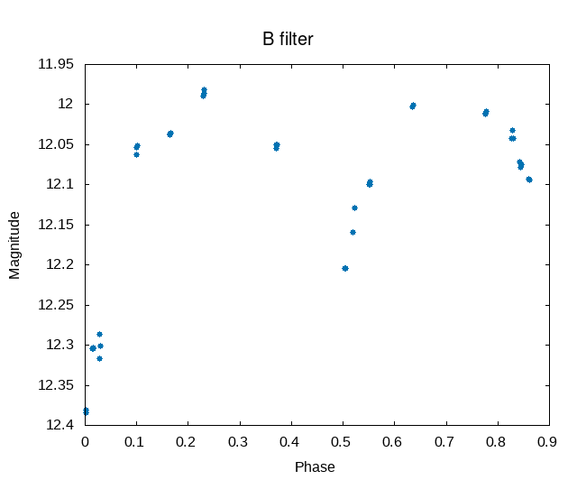
\includegraphics[width=2.5in]{Figures/B.png}
  \end{subfigure} \\
  \begin{subfigure}{}
    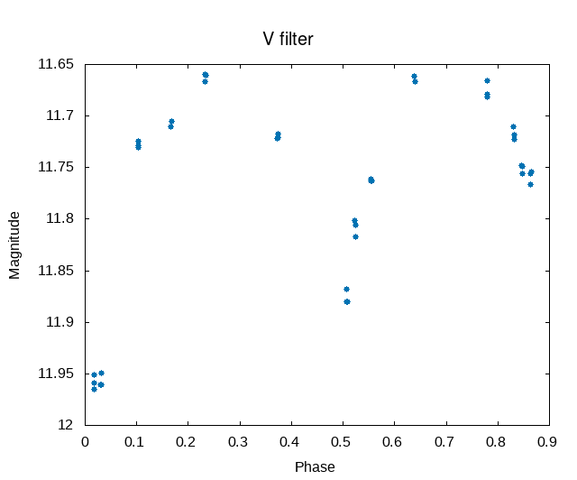
\includegraphics[width=2.5in]{Figures/V.png}
  \end{subfigure}
  \begin{subfigure}{}
    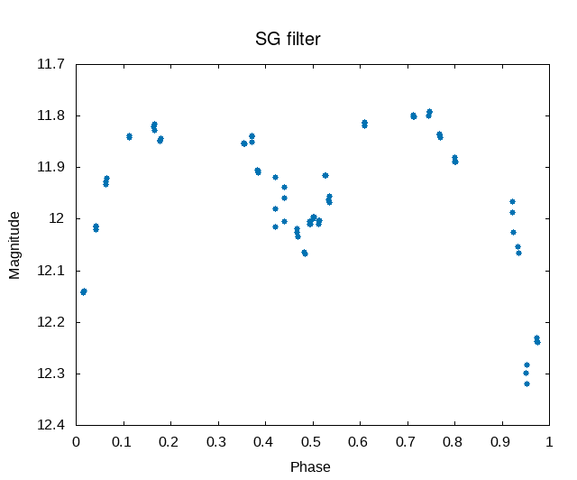
\includegraphics[width=2.5in]{Figures/SG.png}
  \end{subfigure}
  \begin{subfigure}{}
    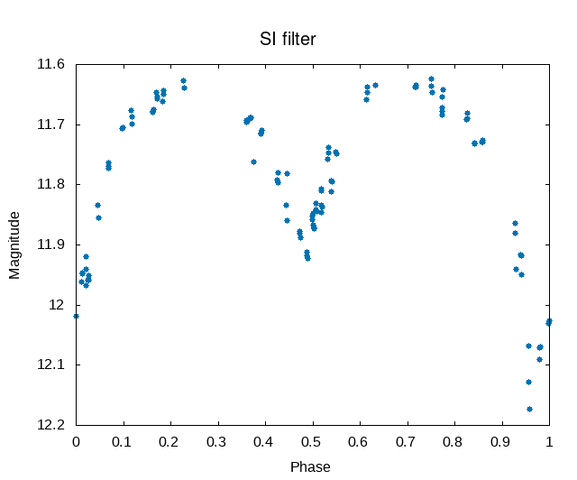
\includegraphics[width=2.5in]{Figures/SI.png}
  \end{subfigure}
  \begin{subfigure}{}
    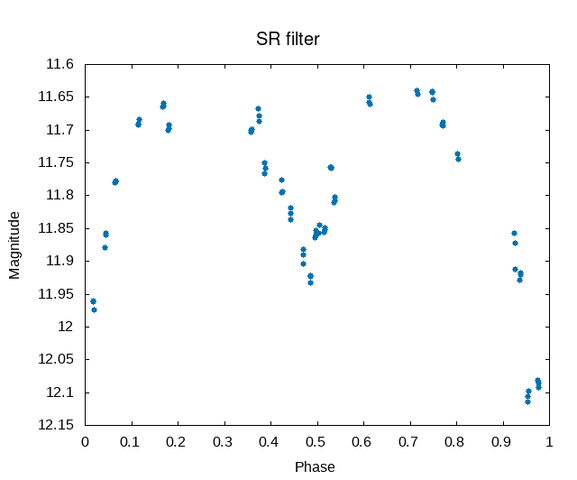
\includegraphics[width=2.5in]{Figures/SR.png}
  \end{subfigure}
  \caption{Light curves of V765 Cas in individual filters.}
  \label{fig:indivlightcurves}
\end{figure}

\bibliography{refs}{}
\bibliographystyle{aasjournal}
\end{document}